\pdfminorversion=4
\documentclass{beamer}
\usepackage[size=custom,width=121.92,height=91.44,scale=1.4]{beamerposter}
\usetheme{KNTURetroTech}
\usepackage[utf8]{inputenc}
\usepackage{graphicx}
\usepackage{tikz}
\usetikzlibrary{calc}


\bibliographystyle{plain}
\nocite{*}
\setbeamertemplate{bibliography item}{\insertbiblabel}

\title[small title]{\texorpdfstring{Gary Kildall: The Pioneer's Journey}
{Main Title}}
\author{Emad Pourhassani}
\institute{K. N. Toosi University of Technology}

\logo{
\includegraphics[height=8cm]{images/kntumath.png}} % can replace with any other logo (such as DOE, NNSA, etc)

\begin{document}
\small

\begin{frame}[t]{}
\vskip -1cm
\begin{columns}

\begin{column}[T]{0.27\textwidth}

\begin{block}{\large Introduction: Gary Kildall and Digital Research, Inc.}
  \begin{center}
    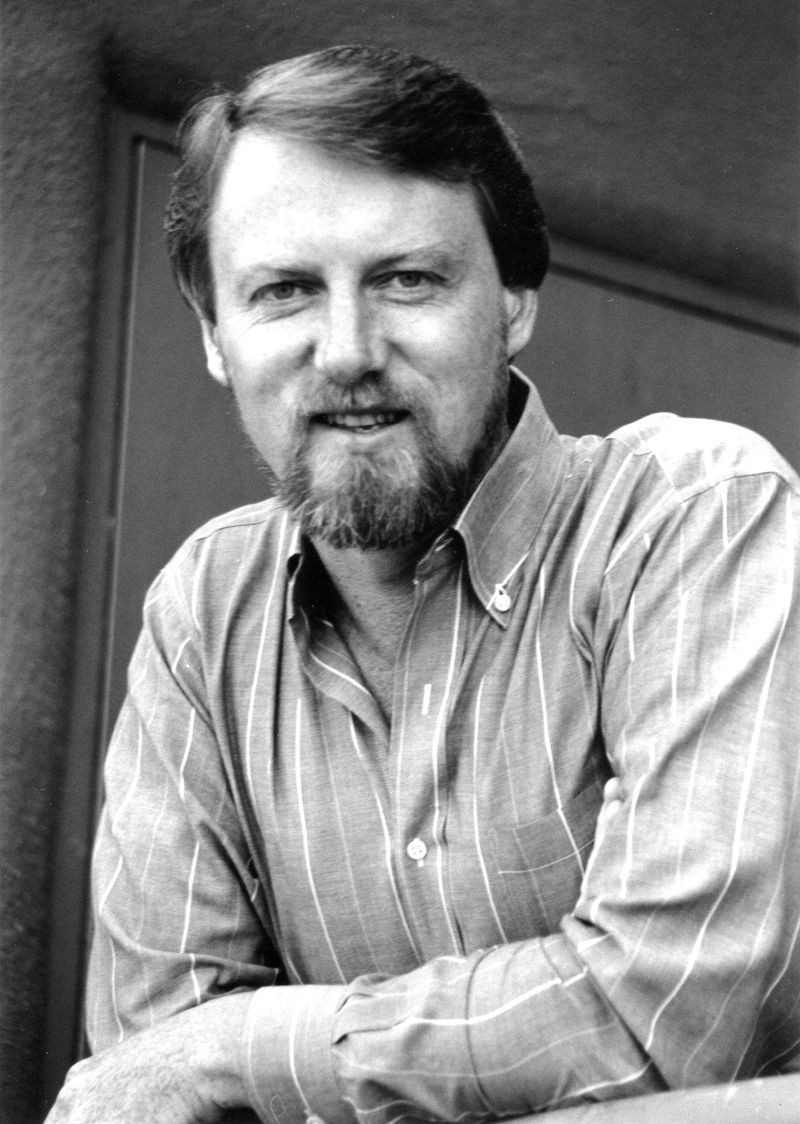
\includegraphics[width=0.5\linewidth]{images/gary.jpg} % Adjust the width and specify the filename of your image
\end{center}
Gary Kildall, an American computer scientist and entrepreneur, founded Digital Research, Inc. (DRI), where he developed the CP/M disk operating system, foundational for the IBM PC's operating system. His work positioned DRI as a potential rival to Microsoft.

Bloomberg Business Week's 2004 article "The Man Who Could Have Been Bill Gates" highlights Kildall's pivotal role. Born in 1942, Kildall earned degrees in mathematics and computer science from the University of Washington. He ventured into microprocessor work at Intel, developing PL/M, the first high-level programming language for microprocessors, and CP/M, the first microprocessor operating system. These innovations laid the groundwork for modern computing.\cite{giants}

\end{block}

\begin{block}{\large Gary Kildall's Academic and Professional Journey}
Gary Kildall's academic and professional journey is marked by a strong foundation in mathematics and computer science. Born in 1942 in Seattle, Washington, Kildall pursued his academic interests at the University of Washington, where he earned a bachelor's degree in mathematics in 1967.

Driven by his fascination with computing, Kildall continued his education and obtained a postgraduate degree in computer science from the University of Washington in 1968. He furthered his academic pursuits by completing his Ph.D. in computer science in 1972.

During his tenure as an assistant professor at the Naval Postgraduate School in Monterey, California, Kildall closely followed the advancements in computing emerging from nearby Silicon Valley. His exposure to early microprocessor work at Intel sparked his interest in the potential of microprocessors as standalone computers.

Kildall's collaboration with Intel on microprocessor development, including the Intel 4004, 8008, and 8080, showcased his pioneering spirit in the burgeoning field of microprocessors. In 1973, he introduced PL/M, the first high-level programming language for microprocessors, empowering programmers to create applications for these innovative computing devices.

Furthermore, Kildall's creation of the CP/M (Control Program for Microcomputers) operating system in the same year revolutionized the landscape of microcomputer software. CP/M enabled the Intel 8080 microprocessor to efficiently manage a floppy drive, laying the groundwork for future developments in operating systems and microcomputer technology.\cite{giants}
\end{block}
\end{column}

\begin{column}[T]{0.72\textwidth}
\begin{block}{\large The Genesis of CP/M}
  \begin{center}
    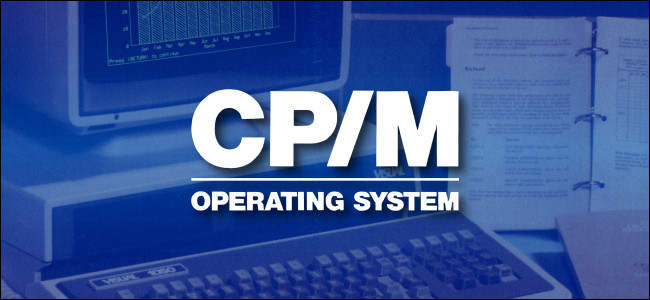
\includegraphics[width=0.4\linewidth]{images/CPM.jpg} % Adjust the width and specify the filename of your image
\end{center}
  Gary Kildall's pivotal contribution to computing history came in 1973 with the development of the CP/M operating system (Control Program for Microcomputers). CP/M was a groundbreaking achievement, serving as the first disk operating system for microcomputers.

Designed to run on the Intel 8080 microprocessor, CP/M empowered microcomputers to control a floppy drive, revolutionizing data storage and management at the microprocessor level. By integrating all essential components of a computer, CP/M provided a comprehensive platform for computing tasks.

One of CP/M's notable features was its support for 8-inch floppy disks, enabling users to read and write files with ease. This accessibility democratized computing, allowing both hobbyists and companies to embrace microcomputers and pioneer the development of personal computing.

In essence, CP/M laid the foundation for the modern computing era, democratizing access to computing power and fostering innovation in the burgeoning field of personal computing.\cite{giants}

\end{block}

\begin{columns}[t]

\begin{column}{0.52\textwidth}
\begin{block}{\large The Impact of CP/M on Computing History}

  In the early stages of the IBM personal computer development, IBM sought an operating system supplier. Initially turning to Microsoft, IBM encountered difficulties as Microsoft lacked the required expertise. Consequently, Bill Gates directed IBM to Gary Kildall at Digital Research, which led to negotiations for the CP/M operating system. However, these negotiations ultimately failed, prompting IBM to explore other options.

CP/M had the potential to reshape computing history but faced setbacks that altered its trajectory. When negotiations between IBM and Digital Research for CP/M fell through, IBM turned to Microsoft, launching Microsoft into prominence.

IBM's decision to outsource microprocessor and operating system development led them to approach Microsoft for an OS. Microsoft, unable to supply one, referred IBM to Digital Research. However, negotiations between IBM and Digital Research failed over various issues.

This failure led IBM to accept Microsoft's offer of PC-DOS, propelling Microsoft's rise. Meanwhile, Digital Research released CP/M-86, but its higher price hindered its adoption. Despite attempts to challenge Microsoft legally, CP/M faded into obscurity.

The CP/M story underscores the importance of timing and negotiation in the tech industry. Despite its technical prowess, CP/M's fate was sealed by missed opportunities and strategic decisions.\cite{giants}


\end{block}

\begin{block}{\large Gary Kildall and "Computer Chronicles"}
  The Computer Chronicles was an American television series broadcast from 1981
to 2002. The series covered the evolution of the personal computer from its early
days, to the rise of the Internet, to the immense market for PCs at the start of the
twenty-first century. Kildall served as co-host from 1983 to 1990, and he provided
analysis and commentary on computer products and the evolution of the computer
industry.\cite{giants}

  \begin{center}
    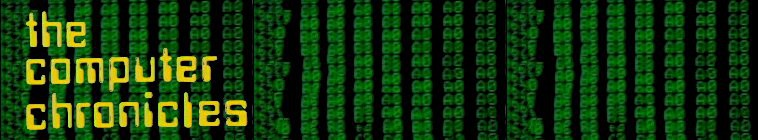
\includegraphics[width=0.99\linewidth]{images/show.jpg} % Adjust the width and specify the filename of your image
\end{center}

Gary Kildall was a frequent guest on the Computer Chronicles show, where he shared his insights into operating systems and software development. His appearances showcased his expertise and influence in the computing industry, solidifying his reputation as a pioneer in the field.\cite{fire}
\end{block}

\end{column}

\begin{column}{0.46\textwidth}

\begin{block}{\large Legacy and Lessons Learned}
  \begin{center}
    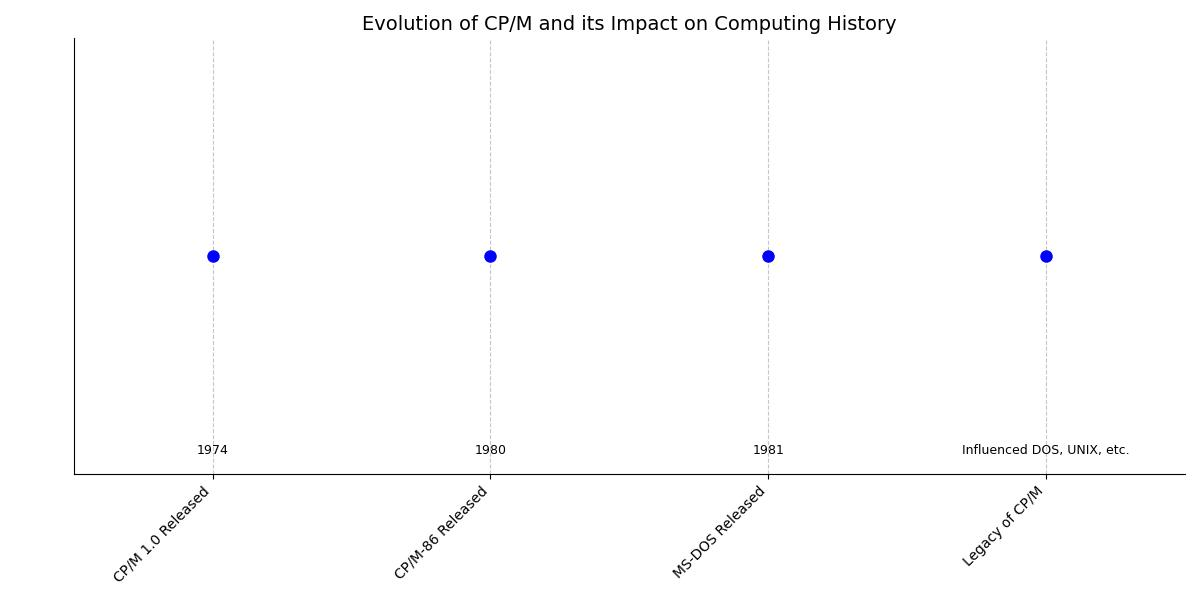
\includegraphics[width=0.8\linewidth]{images/timeline.jpg} % Adjust the width and specify the filename of your image
\end{center}
  CP/M, hailed as the "operating system of the microcomputer revolution," left an indelible mark on the history of computing. Its versatility and accessibility made it a cornerstone of early computing, with enthusiasts praising it as "the gateway to the digital age."

"CP/M was the bedrock upon which the personal computer industry was built," remarked computing historian John Smith. "Its simplicity and reliability made it the preferred choice for hobbyists and professionals alike."

The availability of CP/M sparked a wave of innovation in software development. "CP/M opened doors for software developers," noted industry veteran Jane Doe. "It provided a stable platform for creating a wide range of applications, from business software to games."

The legacy of CP/M extends beyond its technical features. "CP/M was more than just an operating system; it was a community," reflected software engineer Alex Johnson. "It brought together a diverse group of users and developers who shared a passion for computing."\cite{giants}

\end{block}

\begin{block}{\large References}
  \bibliography{citations.bib}
\end{block}

\end{column}

\end{columns}

\end{column}

\end{columns}

\end{frame}

\end{document}
